\univlogo

{\Huge May 15}\vspace{5mm}

\hypertarget{introduction}{%
\subsection{Introduction}\label{introduction}}

\begin{enumerate}
\def\labelenumi{\arabic{enumi}.}
\item
  Calculate explicit probabilities for hypotheses, such as the naive
  Bayes classifier. The most practical approaches to certain types of
  learning problems.
\item
  Bayesian methods provide a useful perspective for understanding many
  learning algorithms that do not explicitly manipulate probabilities.
\end{enumerate}

Feature:

\begin{itemize}
\item
  Each \textbf{observed training example} can incrementally decrease or
  increase the estimated probability that a hypothesis is correct.
\item
  \textbf{Prior knowledge} can be combined with observed data to
  determine the final probability of a hypothesis.
\item
  Bayesian methods can accommodate hypotheses that make
  \textbf{probabilistic predictions}.
\item
  New instances can be classified by combining the predictions of
  \textbf{multiple hypotheses}, weighted by their probabilities.
\item
  In cases where Bayesian methods prove computationally intractable,
  they can provide a standard of \textbf{optimal decision} making
  against which other practical methods can be measured.
\end{itemize}

One practical difficulty:

\begin{itemize}
\item
  Bayesian methods typically require \textbf{initial knowledg}e of many
  probabilities.
\end{itemize}

\hypertarget{bayes-theorem}{%
\subsection{Bayes Theorem}\label{bayes-theorem}}

One way to specify the \emph{best} hypothesis is to say that we demand
the \emph{most probable} hypothesis, given the data \(D\) plus any
initial knowledge about the prior probabilities of the various
hypotheses in space \(H\).

Bayes theorem provides a way to \ul{calculate the probability of a
hypothesis based on its prior probability}, the probabilities of
observing various data given the hypothesis, and the observed data
itself.

Symbols:

\begin{itemize}
\item
  \(P(h)\): \emph{Prior probability}.

  \begin{itemize}
  \item
    The initial probability that hypothesis \(h\) holds, before we have
    observed the training data.
  \item
    Reflecting any background knowledge we have about the chance that
    \(h\) is a correct hypothesis.
  \end{itemize}
\item
  \(P(D)\): The prior probability that training data \(D\) will be
  observed.

  \begin{itemize}
  \item
    The probability of \(D\) given no knowledge about which hypothesis
    holds.
  \end{itemize}
\item
  \(P(D|h)\): The probability of observing data \(D\) given some world
  in which hypothesis \(h\) holds.
\item
  \(P(x|y)\): The probability of \(x\) given \(y\).
\item
  \(P(h|D)\): \emph{posterior probability} of \(h\)

  \begin{itemize}
  \item
    The probability that \(h\) holds given the observed training data
    \(D\).
  \item
    Reflecting our confidence that \(h\) holds after we have seen the
    training data \(D\).
  \item
    Reflecting the influence of the training data \(D\).
  \end{itemize}
\end{itemize}

\textbf{Bayes theorem:}

\[P(h|D)=\cfrac{P(D|h)P(h)}{P(D)}\]

\begin{itemize}
\item
  \(P(h|D)\) increases with \(P(h)\) and with \(P(D|h)\)
\item
  \(P(D|h)\) decreases as \(P(D)\) increases, because the more probable
  it is that \(D\) will be observed independent of \(h\), the less
  evidence \(D\) provides in support of \(h\)
\end{itemize}

\textbf{Maximum a posteriori (MAP)} hypothesis:

\begin{equation*}
  \begin{aligned}
  h_{MAP} &\equiv \underset{h\in H}{\text{argmax}} \, P(h|D) \\
  &= \underset{h\in H}{\text{argmax}} \, \frac{P(D|h)P(h)}{P(D)} \\
  &= \underset{h\in H}{\text{argmax}} \, P(D|h)P(h)
\end{aligned}
\end{equation*}

\begin{quote}
We dropped the term \(P(D)\) because it is a constant independent of
\(h\)
\end{quote}

\textbf{Maximum likelihood (ML)} hypothesis:

\[h_{ML}\equiv \underset{h\in H}{argmax}\ P(D|h)\]

\begin{quote}
In some cases, we will assume that every hypothesis in \(H\) is equally
probable a priori (\(P(h_i)=P(h_j)\) for all \(h_i\) and \(h_j\) in
\(H\)).
\end{quote}

\hypertarget{an-example}{%
\subsubsection{An example}\label{an-example}}

If

\begin{equation*}
\begin{aligned}
&P(cancer)=0.008, &P(\neg cancer)=0.992\\
&P(\oplus |cancer)=0.98, &P(\ominus|cancer)=0.02\\
&P(\oplus|\neg cancer)=0.03, &P(\ominus|\neg cancer)=0.97
\end{aligned}
\end{equation*}

Then

\begin{equation*}
\begin{aligned}
P(\oplus |cancer)P(cancer)=0.98\times0.008=0.0078&(\oplus\ and\ cancer)\\
P(\oplus|\neg cancer)P(\neg cancer)=0.03\times0.992=0.0298&(\oplus\ but\ no\ cancer)
\end{aligned}
\end{equation*}

\hypertarget{bayes-theorem-and-concept-learning}{%
\subsection{Bayes Theorem and Concept
Learning}\label{bayes-theorem-and-concept-learning}}

\hypertarget{brute-force-bayes-concept-learning}{%
\subsubsection{BRUTE-FORCE Bayes Concept
Learning}\label{brute-force-bayes-concept-learning}}

Consider:

\begin{itemize}
\item
  Target concept: \(c:X\rightarrow\{0,1\}\)
\item
  Training examples: \(<<x_1,d_1>...<x_m,d_m>>\), where \(x_i\) is some
  instance from \(X\) and where \(d_i\) is the target value of \(x_i\).
\end{itemize}

BRUTE\_FORCE MAP learning algorithm

\begin{enumerate}
\def\labelenumi{\arabic{enumi}.}
\item
  For each hypothesis \(h\) in \(H\), calculate the posterior
  probability

  \[p(h|D)=\cfrac{P(D|h)P(h)}{P(D)}\]
\item
  Output the hypothesis \(h_{MAP}\) with the highest posterior
  probability

  \[h_{MAP}=\underset{h\in H}{argmax}\ P(h|D)\]
\end{enumerate}

We must specify what values are to be used for \(P(h)\) and for
\(P(D|h)\) (\(P(D)\) will be determined once we choose the other two).

Assumptions:

\begin{enumerate}
\def\labelenumi{\arabic{enumi}.}
\item
  The training data \(D\) is \ul{noise free}.
\item
  The target concept \(c\) is contained in the hypothesis space \(H\).
\item
  We have no a priori reason to believe that any hypothesis is more
  probable than any other.
\end{enumerate}

Given these assumptions:

\[P(h)=\cfrac{1}{|H|}\, for\ all\ h\ in\ H\\\]

Since the training data is noise free: the probability of observing
classification \(d_i\) given \(h\) is just 1 if \(d_i=h(x_i)\) and 0 if
\(d\neq h(x_i)\).

\[P(D|h)=\begin{cases}
1 & \text{if }d_i=h(x_i)\text{ for all }d_i\text{ in }D\\
0 & \text{otherwise} 
\end{cases}\]

So we have:

\begin{equation*}
\begin{aligned}
P(h|D)&=&\cfrac{1\cdot\cfrac{1}{|H|}}{P(D)}&\\
&=&\cfrac{1\cdot\cfrac{1}{|H|}}{\cfrac{|VS_{H,D}|}{|H|}}&\\
&=&\cfrac{1}{|VS_{H,D}|} &\text{ if }h\text{ is consistenwith }D\
\end{aligned}
\end{equation*}


where \(VS_{H,D}\), is the subset of hypotheses from \(H\) that are
consistent with \(D\).

So

\begin{equation*}
\begin{aligned}
P(D)&=&\sum_{h_i\in H}P(D|h_i)P(h_i)\\
&=&\sum_{h_i\in VS_{H,D}}1\cdot \cfrac{1}{|H|}+\sum_{h_i\notin VS_{H,D}}0\cdot\cfrac{1}{|H|}\\
&=&\cfrac{|VS_{H,D}|}{|H|}
\end{aligned}
\end{equation*}


To summarize, the posterior probability \(P(h|D)\) under our assumed
\(P(h)\) and \(P(D|h)\) is:

\[P(h|D)=\begin{cases}
\cfrac{1}{|VS_{H,D}|} & \text{if }h\text{ is consistent with }D\\
0 & \text{otherwise}
\end{cases}\]

Initially all hypotheses have the same probability. As training data
accumulates, the posterior probability for inconsistent hypotheses
becomes zero while the total probability summing to one is shared
equally among the remaining consistent hypotheses.


\begin{figure}[H]
  \centering
  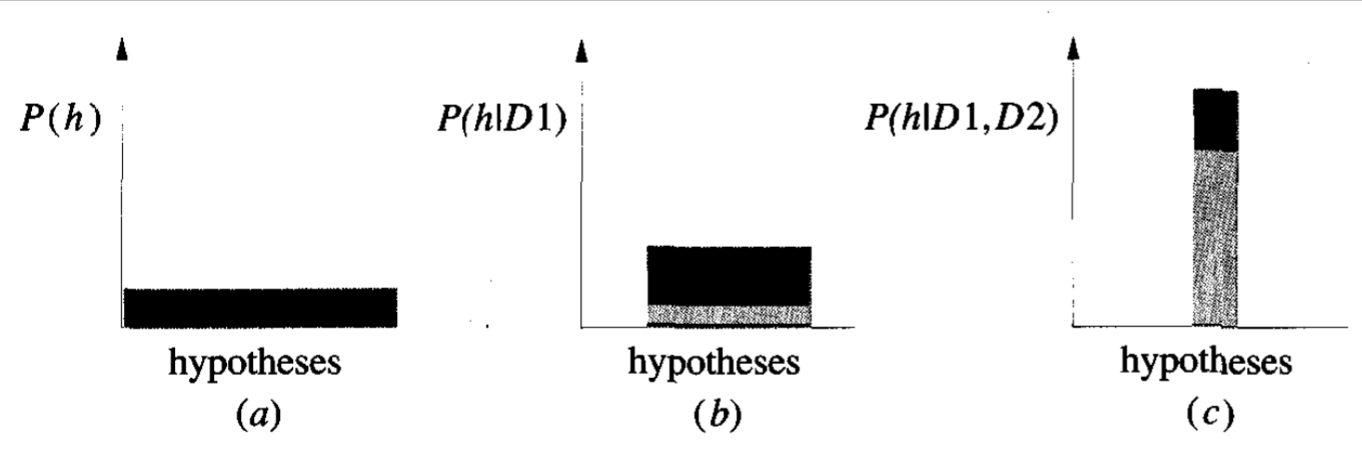
\includegraphics[width=1\textwidth]{./2023May/MAP.png}
  \caption{Maximum a Posteriori}
  \label{MAP}
\end{figure}

\hypertarget{map-hypotheses-and-consistent-learners}{%
\subsubsection{MAP Hypotheses and Consistent
Learners}\label{map-hypotheses-and-consistent-learners}}

Every consistent learner outputs a MAP hypothesis, if we assume a
\ul{uniform} prior probability distribution over \(H\), and if we assume
\ul{deterministic}, \ul{noise-free} training data.

The Bayesian framework allows one way to characterize the behavior of
learning algorithms, even when the learning algorithm does not
explicitly manipulate probabilities.

\hypertarget{maximum-likelihood-and-least-squared-error-hypotheses}{%
\subsection{Maximum Likelihood and Least-Squared Error
Hypotheses}\label{maximum-likelihood-and-least-squared-error-hypotheses}}

Continuous-valued target function-a problem faced by many learning
approaches such as neural network learning, linear regression, and
polynomial curve fitting.

A straightforward Bayesian analysis will show that \emph{under certain
assumptions any learning algorithm that minimizes the squared error
between the output hypothesis predictions and the training data will
output a maximum likelihood hypothesis}.

Consider:

\begin{itemize}
\item
  Learner \(L\)
\item
  Instance space \(X\)
\item
  Hypothesis space \(H\)
\item
  Function \(h:X\rightarrow\mathfrak{R}\), where \(\mathfrak{R}\)
  represents the set of real numbers
\item
  Problem: Learn an unknown target function
  \(f:X\rightarrow\mathfrak{R}\) drawn from \(H\)
\item
  A set of \(m\) training examples is provided, where the target value
  of each example is corrupted by random noise drawn according to a
  Normal probability distribution.

  \begin{quote}
  Each training example is a pair of the form \(<x_i,d_i>\) where
  \(d_i=f(x_i)+e_i\). Here \(f(x_i)\) is the noise-free value of the
  target function and \(e_i\) is a random variable representing the
  noise.
  \end{quote}
\item
  Task: To output a maximum likelihood hypothesis, or, equivalently, a
  MAP hypothesis assuming all hypotheses are equally probable a priori.
\end{itemize}

\[h_{ML}=\underset{h\in H}{argmax}\ p(D|h)\]

Assuming the training examples are mutually independent given \(h\):

\[h_{ML}=\underset{h\in H}{argmax}\ \prod_{i=1}^{m}p(d_i|h)\]

Given that \(e_i\sim N(\mu, \sigma^2)\), then
\(d_i\sim N(f(x_i),\sigma^2)\). Therefore \(p(d_i|h)\) can be written as
a Normal distribution with variance \(\sigma^2\) and mean
\(\mu=f(x_i)\):

\begin{equation*}
\begin{aligned}
p(d_i|h)&=\cfrac{1}{\sqrt{2\pi\sigma^2}}e^{-\cfrac{1}{2\sigma^2}(d_i-\mu)^2}\\
&=\cfrac{1}{\sqrt{2\pi\sigma^2}}e^{-\cfrac{1}{2\sigma^2}(d_i-f(x_i))^2}
\end{aligned}
\end{equation*}

And we are writing the expression for the probability of \(d_i\) given
that \(h\) is the correct description of the target function \(f\), so
\(\mu=f(x_i)=h(x_i)\), yielding:

\begin{equation*}
\begin{aligned}
h_{ML}&=\underset{h\in H}{argmax}\ \prod_{i=1}^{m}\cfrac{1}{\sqrt{2\pi\sigma^2}}e^{-\cfrac{1}{2\sigma^2}(d_i-\mu)^2}\\
&=\underset{h\in H}{argmax}\ \prod_{i=1}^{m}\cfrac{1}{\sqrt{2\pi\sigma^2}}e^{-\cfrac{1}{2\sigma^2}(d_i-h(x_i))^2}
\end{aligned}
\end{equation*}


We choose to maximize its logarithm:

\[h_{ML}=\underset{h\in H}{argmax}\ \sum_{i=1}^{m}\ln\cfrac{1}{\sqrt{2\pi\sigma^2}}-\cfrac{1}{2\sigma^2}(d_i-h(x_i))^2\]

The first term is a constant so:

\[h_{ML}=\underset{h\in H}{argmax}\ \sum_{i=1}^{m}-\cfrac{1}{2\sigma^2}(d_i-h(x_i))^2\\
=\underset{h\in H}{argmin}\ \sum_{i=1}^{m}\cfrac{1}{2\sigma^2}(d_i-h(x_i))^2\]

Discard constants that are independent of \(h\):

\[h_{ML}=\underset{h\in H}{argmin}\ \sum_{i=1}^{m}(d_i-h(x_i))^2\]

\begin{quote}
\begin{itemize}
\item
  As the above derivation makes clear, the squared error term
  \((d_i-h(x_i))^2\) follows directly from the exponent in the
  definition of the Normal distribution.
\item
  Similar derivations can be performed starting with other assumed noise
  distributions, producing different results.
\end{itemize}
\end{quote}

\begin{quote}
The above analysis considers noise only in the \emph{target value} of
the training example and does not consider noise in the \emph{attributes
describing the instances themselves}.
\end{quote}

\hypertarget{maximum-likelihood-hypotheses-for-predicting-probabilities}{%
\subsection{Maximum Likelihood Hypotheses for Predicting
Probabilities}\label{maximum-likelihood-hypotheses-for-predicting-probabilities}}

Treating both \(x_i\) and \(d_i\) as random variables, and assuming that
each training example is drawn independently, we can write \(P(D|h)\) as

\[P(D|h)=\prod_{i=1}^mP(x_i,d_i|h)\]

Assuming \(x_i\) is independent of the hypothesis \(h\):

\[P(D|h)=\prod_{i=1}^mP(x_i,d_i|h)=\prod_{i=1}^mP(d_i|h,x_i)P(x_i)\]

\(P(d_i=1|h,x_i)=h(x_i)\), and in general:

\begin{equation*}
\begin{aligned}
P(d_i|h,x_i)&=\begin{cases}
h(x_i) & \text{if }d_i=1\\
1-h(x_i) & \text{if }d_i=0
\end{cases}\\
&=h(x_i)^{d_i}(1-h(x_i))^{1-d_i}
\end{aligned}
\end{equation*}

So the expression for the \ul{maximum likelihood hypothesis} is:

\[h_{ML}=\underset{h\in H}{argmax}\prod_{i=1}^mh(x_i)^{d_i}(1-h(x_i))^{1-d_i}P(x_i)\]

Drop the independent constant:

\[h_{ML}=\underset{h\in H}{argmax}\prod_{i=1}^mh(x_i)^{d_i}(1-h(x_i))^{1-d_i}\]

Looks like a generalization of the \emph{Binomial distribution}. It will
be easier to work with the log of the likelihood, yielding:

\[h_{ML}=\underset{h\in H}{argmax}\sum_{i=1}^m(d_i\ln h(x_i)+(1-d_i)\ln(1-h(x_i)))\]

The negation of the above quantity is sometimes called the \emph{cross
entropy}.

\hypertarget{minimum-description-length-principle}{%
\subsection{Minimum Description Length
Principle}\label{minimum-description-length-principle}}

Minimum Description Length (MDL)

Consider:

\[h_{MAP}=\underset{h\in H}{argmax}\ P(D|h)P(h)\]

equivalently expressed in terms of maximizing the \(log_2\)

\begin{equation*}
\begin{aligned}
  h_{MAP}&=&\underset{h\in H}{argmax}\ \log_2P(D|h)+\log_2P(h)\\
  &=&\underset{h\in H}{argmin}\ -\log_2P(D|h)-\log_2P(h)
\end{aligned}
\end{equation*}


Interpret equation above from \textbf{coding theory}:

\begin{itemize}
\item
  \(-\log_2P(h)\) is the description \underline{length of \(h\)} under the
  optimal encoding for the hypothesis space \(H\).
\item
  \(-\log_2P(D|h)\) is the description l\underline{ength of the training data
  \(D\)} given hypothesis \(h\).

  \begin{quote}
  \(L_{C_{D|H}}(D|h)=-\log_2P(D|h)\)
  \end{quote}
\item
  So

  \[h_{MAP}=\underset{h}{argmin}\ L_{C_H}(h)+L_{C_{D|h}}(D|h)\]

  where \(C_H\) and \(C_{D|h}\) are the optimal encodings for \(H\) and
  for \(D\) given \(h\).
\end{itemize}

\textbf{Minimum Description Length principle}: Choose \(h_{MDL}\) where:

\[h_{MDL}=\underset{h\in H}{argmin}\ L_{C_1}(h)+L_{C_2}(D|h)\]

\begin{quote}
If we choose \(C_1\) to be the optimal encoding of hypotheses \(C_H\),
and if we choose \(C_2\) to be the optimal encoding \(C_{D|h}\), then
\(h_{MDL}=h_{MAP}\).
\end{quote}

\hypertarget{bayes-optimal-classifier}{%
\subsection{Bayes Optimal Classifier}\label{bayes-optimal-classifier}}

\begin{itemize}
\item
  Three hypothesis: \(h_1,h_2,h_3\)
\item
  Posteriori probabilities of these hypotheses: 0.4, 0.3, 0.3
\item
  \(h_1\) is the MAP hypothesis.
\item
  A new instance \(h\) is encountered, classified positive by \(h_1\)
  but negative by \(h_2\) and \(h_3\).
\item
  Taking all hypotheses into account, the probability that \(x\) is
  positive is 0.4 and the probability that it is negative is therefore
  0.6.
\end{itemize}

The most probable classification of the new instance is obtained by
combining the predictions of all hypotheses, \ul{weighted by their
posterior probabilities}.

\[P(v_j|D)=\sum_{h_i\in H}P(v_j|h_i)P(h_i|D)\]

\textbf{Bayes optimal classification}:

\[\underset{v_j\in V}{argmax}\sum_{h_i\in H}P(v_j|h_i)P(h_i|D)\]

\begin{quote}
The set of the new instance is \(V=\{\oplus|,\ominus\}\), and

\begin{equation*}
\begin{aligned}
P(h_1|D)=0.4,&P(\ominus|h_1)=0,&P(\oplus|h_1)=1\\
P(h_2|D)=0.3,&P(\ominus|h_2)=1,&P(\oplus|h_2)=0\\
P(h_3|D)=0.3,&P(\ominus|h_3)=1,&P(\oplus|h_3)=0
\end{aligned}
\end{equation*}


therefore

\[\sum_{h_i\in H}P(\oplus|h_i)P(h_i|D)=0.4\\
\sum_{h_i\in H}P(\ominus|h_i)P(h_i|D)=0.6\]

and

\[\underset{v_j\in\{\oplus|,\ominus\}}{argmax}\sum_{h_i\in H}P(v_j|h_i)P(h_i|D)=\ominus\]
\end{quote}

No other classification method using the same hypothesis space and same
prior knowledge can outperform this method on average. This method
maximizes the probability that the new instance is classified correctly,
given the available data, hypothesis space, and prior probabilities over
the hypotheses.

\hypertarget{gibbs-algorithm}{%
\subsection{Gibbs Algorithm}\label{gibbs-algorithm}}

It can be quite \textbf{costly} to apply Bayes optimal classifier. An
\textbf{alternative, less optimal} method is Gibbs algorithm.

\begin{itemize}
\item
  Choose a hypothesis \(h\) from \(H\) \ul{at random}, according to the
  \ul{posterior probability} distribution over \(H\)
\item
  Use \(h\) to predict the classification of the next instance \(x\).
\end{itemize}

Under certain conditions the expected misclassification error for the
Gibbs algorithm is at most \textbf{twice} the expected error of the
Bayes optimal classifier.

It implies that if the learner assumes a uniform prior over \(H\), and
if target concepts are in fact drawn from such a distribution when
presented to the learner, \ul{then classifying the next instance according to a hypothesis drawn at random from the current version space (according to a uniform distribution), will have expected error \textbf{at most twice} that of the Bayes optimal classifier}.

\hypertarget{naive-bayes-classifier}{%
\subsection{Naive Bayes Classifier}\label{naive-bayes-classifier}}

The Bayesian approach to classifying the new instance is to assign the
most probable target value \(v_{MAP}\), given the attribute values
\(<a_1,a_2,...,a_n>\) that describe the instance.

\[v_{MAP}=\underset{v_j\in V}{argmax}P(v_j|a_1,a_2,..,a_n)\]

Use Bayes theorem to rewrite this expression as:

\begin{equation*}
\begin{aligned}
v_{MAP}&=\underset{v_j\in V}{\text{argmax}}\cfrac{P(a_1,a_2,..,a_n|v_j)P(v_j)}{P(a_1,a_2,..,a_n)}\\
&=\underset{v_j\in V}{\text{argmax}}P(a_1,a_2,..,a_n|v_j)P(v_j)
\end{aligned}
\end{equation*}

Now we need to estimate the two terms above. It is easy to estimate each
of the \(P(v_j)\) simply by counting the frequency with which each
target value \(v_j\) occurs in the training data. \ul{However, estimating the different} \(P(a_1,a_2,...,a_n|v_j)\) \ul{terms in this fashion is not feasible unless we have a very very large set of training data.}

The naive Bayes classifier is based on the simplifying
\textbf{assumption} that \ul{the attribute values are conditionally
independent given the target value}:

\[P(a_1,a_2,...,a_n|v_j)=\prod_i P(a_i|v_j)\]

\textbf{Naive Bayes classifier}:

\[v_{NB}=\underset{v_j\in V}{argmax}P(v_j)\prod_i P(a_i|v_j)\]

where \(v_{NB}\) denotes the target value output by the naive Bayes
classifier.

To summarize, the naive Bayes learning method involves a learning step
in which the various \(P(v_j)\) and \(P(a_i|v_j)\) terms are estimated,
based on their frequencies over the training data.

\end{document}